\chapter{Implementation}

\section{Simulator Introduction: Qrsim}
QRSim \cite{denardi2013rn} is a multi-vehicle software simulator developed at Department of Computer Science, University College London. QRSim allows a set of UAVs to communicate and cooperate to achieve common goals. It simulates the dynamics of the UAVs as well as the sensors (GPS, IMU, camera) and the inaccuracies in the sensors and environment (e.g. wind, GPS errors). The simulator also includes the implementation of some specific task scenarios. For example, a pursue evasion game, a search and rescue mission etc. The simulator is specifically helpful in simulating general higher-level tasks that involve multiple platforms which sense and react in their environment. The QRSim has been implemented in MATLAB and the source code is available on GitHub \cite{qrsim_github} under modified BSD license.

We now present a brief overview of the main concepts of the simulator and the relevant classes in its implementation \cite{qrsim_github_manual}.

\paragraph{Platforms and Environment Objects}
\textbf{Platforms} represent quadrotor dynamics and sensor models and other platform specific phenomena like aerodynamic turbulence. Platforms subclass the abstract class Platform (defined in \emph{/qrsim/platforms/Platform.m})

\textbf{Environment objects} represent the phenomena that have a direct or indirect impact of the platforms but are not specific to the platforms like wind or the satellite vehicles of the GPS system or the obstacles in the flight path. Environment objects subclass \emph{EnvironmentObject} (defined in \emph{/qrsim/environment}).
\paragraph{State:} State class maintains the state of all the objects taking part in the simulation. For example, the state structure stores variables like 'the simulator time (\emph{t})', 'pseudo-random number generator streams (\emph{rStreams})', 'the simulator time step (\emph{DT})', 'the handle to the 3D graphics visualization (\emph{display3D})'.
\paragraph{Steppable:} Steppable is an abstract class that represents every object that evolves with time. For example, the location of UAV updates after each time quantum (\emph{DT}). Hence the method \emph{step()} exposed by the Steppable class is called which called \emph{update()} on the UAV.
\paragraph{Task:}
Task class allows defining a variety of UAV scenarios and the various objectives for the platforms. The Task class provides a way to derive task objects that specify a scenario and an activity. It exposes methods like \emph{init()}, \emph{updateReward()}, \emph{reward()}, \emph{reset()} and \emph{step()}.
\paragraph{Other abstract classes:}
QRSim API defines several other abstract classes like \emph{AerodynamicTurbulence}, \emph{Sensors}, \emph{AHARS}, \emph{OrientationEstimator}, \emph{Gyroscope}, \emph{Altmeter}, \emph{Accelerometer}.

The main QRSim class defines methods to initialize, set up and control the simulator, namely (a). \emph{init('taskName')} (b) \emph{qrsim.reset()} (c) \emph{qrsim.resetSeed()} (d) \emph{step(U)}.

\section{Qrsim Extensions}

To simulate the message routing protocol and the plume wrapping mission, we had to add/extend some features. In this section, we describe our additions/extensions and our rationale behind our decisions.
\subsection{Message transmission delay}
The QRSim simulator updates the simulation state after one time-quantum (DT) has passed. DT is a configurable parameter with the default value of 0.2 seconds. Below we present an estimate of the propagation delay, experimental setup and data on the message processing delay (transmission + reception) on a BeagleBone Black device.
\begin{figure}[hbtp]
\centering
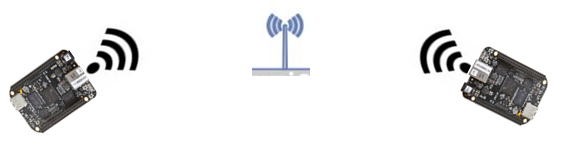
\includegraphics[width=0.8\textwidth]{Chapter-4/figs/beaglebone}
\caption{Measuring processing delay on BeagleBone Black}
\label{fig:proc_delay_setup}
\end{figure}
The setup in \fref{fig:proc_delay_setup} is similar to the configuration proposed in \cite{1378257} to measure network processing delay.

\begin{figure}[hbtp]
\centering
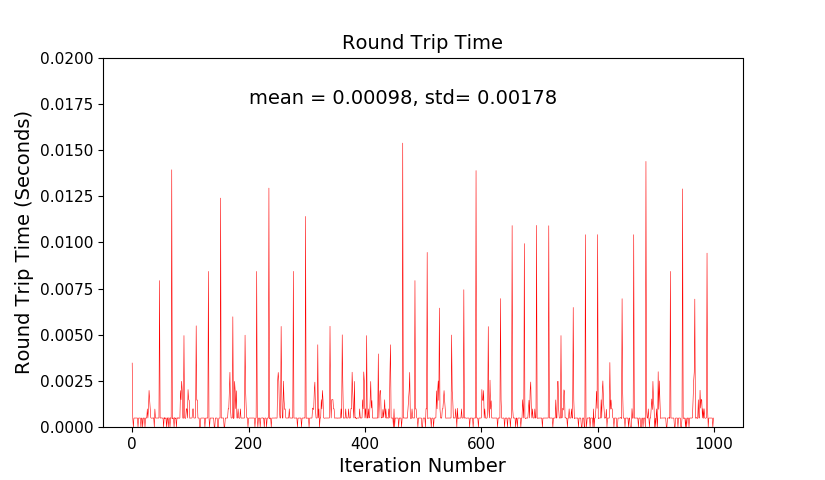
\includegraphics[width=0.8\textwidth]{Chapter-4/figs/transmission_time}
\caption{Round trip time between two BeagleBone Black}
\label{fig:proc_delay_graph}
\end{figure}

A sample plot of round trip time over 1000 iterations is shown in \fref{fig:proc_delay_graph}. It becomes evident that the total message processing delay is much smaller to the time step. Hence, in our simulation, a message transmitted in the time quantum 'x' is also received in the same time quantum 'x'.

\subsection{Radio propagation model}
Our propagation model is based on free space model derived from the Friis transmission formula. \cite{5735774}

The received signal strength $R$ can be calculated as 
\begin{equation}
    R = T - L + N
\end{equation} 
Where,
\begin{itemize}
    \item $R : $ Signal strength at the receiver.
    \item $T : $ Signal strength at the transmitter. (Can be different for each UAV)
    \item $L : $ Path Loss
    \item $N : $ Normal random variable with mean $0$ and standard deviation $\sigma$
\end{itemize}
And Path Loss ($L$) is calculated by the free space path loss equation.
\begin{equation}
 L (dB) = 20 * log_{10} d + 20 * log_{10}(f) + 32.44 - Ft_x - Gr_x 
\end{equation}
Where
\begin{itemize}
    \item $d : $ the distance between the transmitter and receiver (Km)
	\item $f : $ the frequency of transmission (MHz)
    \item $Gt_x : $ the transmitter antenna gain 
    \item $Gr_x : $ the receiver antenna gain.
\end{itemize}

Thereafter, Message Reception Probability $(r) = P(R > R_{th})$. Where $r_{th}$ is the threshold for successful reception of a message. Appropriate values of $T, R, R_{th}$ can be plugged in from the data sheet of WL18xxMOD WiLink\texttrademark Wi-Fi\textregistered   \cite{wilink} (section 5.6 and 5.7) used in BeagleBone black.

\begin{figure}[hbtp]
\centering
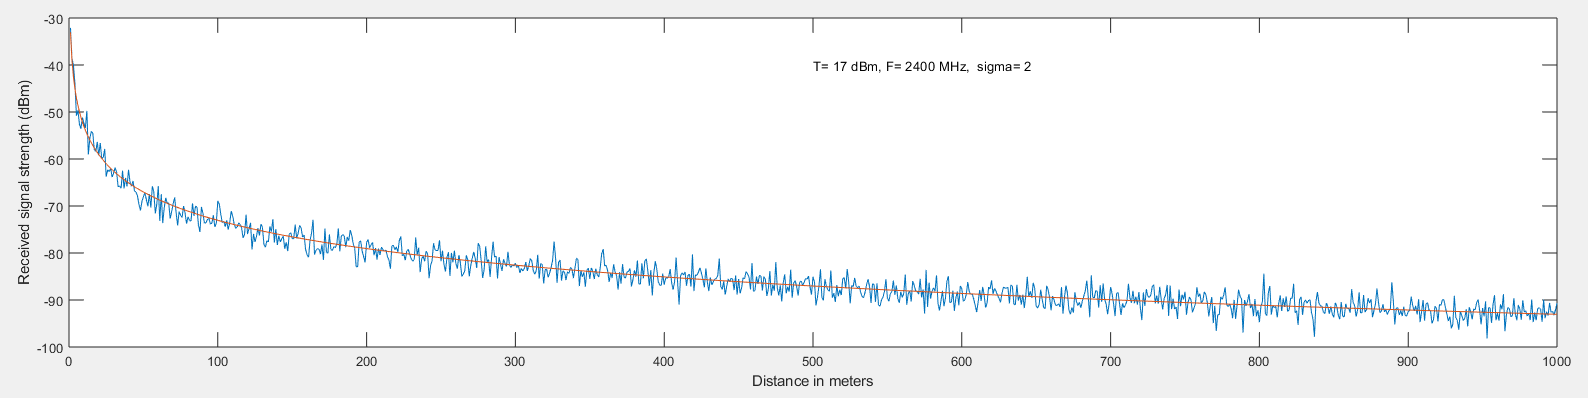
\includegraphics[width=1\textwidth]{ncsuthesis-0.6/Chapter-4/figs/signal_strength}
\caption{Received signal strength vs distance}
\label{fig:signal_strength}
\end{figure}
\begin{figure}[hbtp]
\centering
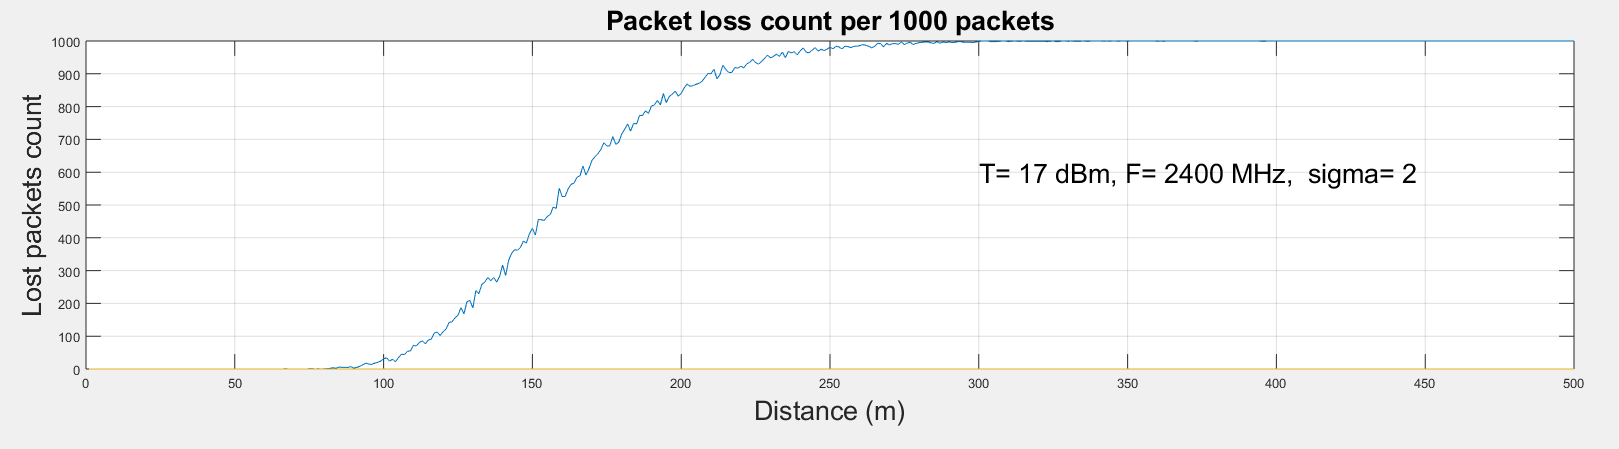
\includegraphics[width=1\textwidth]{ncsuthesis-0.6/Chapter-4/figs/packet_loss}
\caption{Packet loss vs distance}
\label{fig:packet_loss}
\end{figure}
The values used in our simulation are mentioned below and the corresponding received signal strength plots and packet loss plot are shown in \fref{fig:signal_strength} and \fref{fig:packet_loss}:

\begin{eqnarray*}
\begin{aligned}
    & T = 17.1  dBm \\
    & R_{th} = -87.2 dBm \\ 
    & f = 2400 MHz \\
    & \sigma = 2 \\
\end{aligned}
\end{eqnarray*}


\subsection{Inter-UAV attractive and repulsive force function}
The UAVs are initially arranged in a grid and then this grid is maintained during the mission. To maintain the grid formation whenever two UAVs, go out of a certain range, they exert a virtual pull towards each other, and when they come too close they exert a virtual push towards each other. Moreover, once two UAVs are beyond a certain limit, their influence should gradually wear off. We use the following sigmoid function to calculate the push or pull force. 

\begin{equation}
    Y = \frac{X}{1 + |X|}
\end{equation}
\begin{figure}
\centering
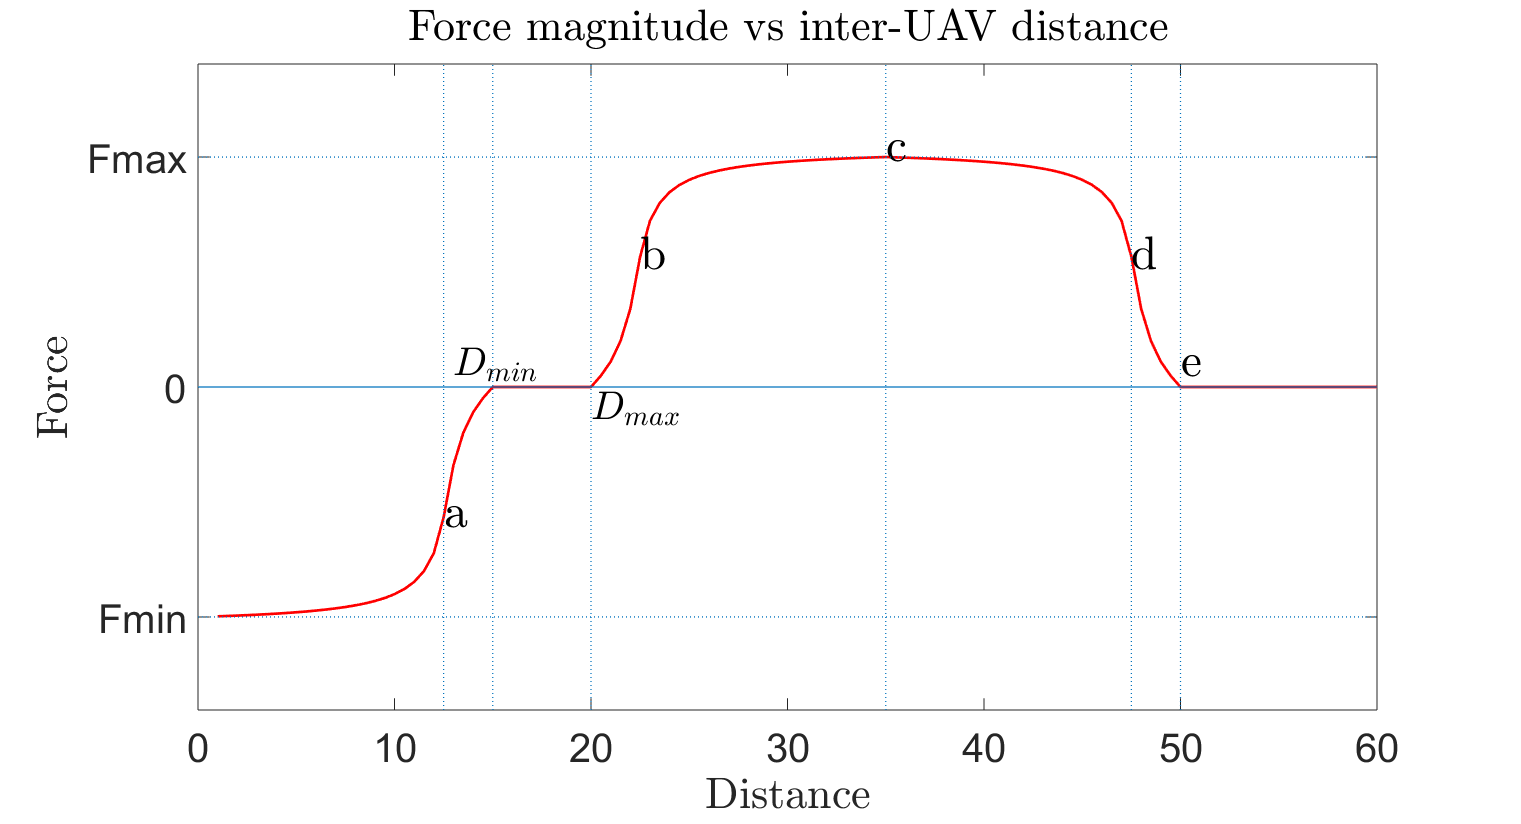
\includegraphics[width=1\textwidth]{ncsuthesis-0.6/Chapter-4/figs/force_function}
\caption{Inter UAV force vs distance}
\label{fig:force_fn}
\end{figure}
Figure \fref{fig:force_fn} shows plot the force magnitude as a function of distance.

\subsection{Location service} \label{loc_service_impl}
\section{Routing Protocol Implementation}
\subsection{Unicast to a UAV}
\subsection{Geocast to a region}
